% VLDB template version of 2020-08-03 enhances the ACM template, version 1.7.0:
% https://www.acm.org/publications/proceedings-template
% The ACM Latex guide provides further information about the ACM template

\documentclass[sigconf, nonacm]{acmart}
\usepackage{algorithm,algpseudocode,float}
\usepackage{lipsum}

\makeatletter
\newenvironment{breakablealgorithm}
  {% \begin{breakablealgorithm}
   \begin{center}
     \refstepcounter{algorithm}% New algorithm
     \hrule height.8pt depth0pt \kern2pt% \@fs@pre for \@fs@ruled
     \renewcommand{\caption}[2][\relax]{% Make a new \caption
       {\raggedright\textbf{\ALG@name~\thealgorithm} ##2\par}%
       \ifx\relax##1\relax % #1 is \relax
         \addcontentsline{loa}{algorithm}{\protect\numberline{\thealgorithm}##2}%
       \else % #1 is not \relax
         \addcontentsline{loa}{algorithm}{\protect\numberline{\thealgorithm}##1}%
       \fi
       \kern2pt\hrule\kern2pt
     }
  }{% \end{breakablealgorithm}
     \kern2pt\hrule\relax% \@fs@post for \@fs@ruled
   \end{center}
  }
\makeatother
%% The following content must be adapted for the final version
% paper-specific
\newcommand\vldbdoi{XX.XX/XXX.XX}
\newcommand\vldbpages{XXX-XXX}
% issue-specific
\newcommand\vldbvolume{14}
\newcommand\vldbissue{1}
\newcommand\vldbyear{2020}
% should be fine as it is
\newcommand\vldbauthors{\authors}
\newcommand\vldbtitle{\shorttitle} 
% leave empty if no availability url should be set
\newcommand\vldbavailabilityurl{http://vldb.org/pvldb/format_vol14.html}
% whether page numbers should be shown or not, use 'plain' for review versions, 'empty' for camera ready
\newcommand\vldbpagestyle{plain} 

\begin{document}
\title{Final Report for Gomoku Project}

%%
%% The "author" command and its associated commands are used to define the authors and their affiliations.
\author{Zhi-Jie Zhang}
\affiliation{
}
\email{18307130184@fudan.edu.cn}

\author{Wen-Bo Du}
\affiliation{
}
\email{18307110359@fudan.edu.cn}


%%
%% The abstract is a short summary of the work to be presented in the
%% article.
\begin{abstract}
%
\quad We implemented several Gomoku AIs by using Monte Carlo tree search, self-teaching Adaptive Dynamic Programming, and improved the adversarial game tree search with $\alpha$-$\beta$ pruning by adding some new technologies. 
%
In details, HMCTS and UCT, two different kinds of Monte Carlo tree search, are both implemented. From the experiment result we can know that HMCTS's performance is better than UCT's, but HMCTS is much more time consuming than UCT. 
%
As to ADP(adaptive dynamic programming), limited by the machine and training time, it doesn't perform as expected, but it is believed that more training time can make a smarter agent.
%
Besides, we improve the adversarial game tree search with $\alpha$-$\beta$ pruning by adding hash index and checkmate search, acting in concert with a depth-7 search tree, the agent performs much more smarter and quicker, and as a result, it finally get at most 1447 rating under Bayesian Elo.

\end{abstract}

\maketitle

%%% VLDB block end %%%

\section{Introduction}

\quad Gomoku is a board game that originated from one of the
various kinds of black and white chess games in ancient China.
%
Nowadays, it has become a popular game played in many places
of the world. A sufficient amount of black or white pieces are
offered to each player. 
%
The players in turns place one piece on the
board. 
%
The winner is the first who forms a line of at least five
adjacent pieces of his color, in horizontal, vertical or diagonal
directions on the board. 
%
Such winning line is called five-in-a-row
which is also referred to the name of the game Gomoku.  

There are quantities of algorithms proposed to implement a Gomoku agent.
%
The most classic algorithms is the game tree search algorithm with $\alpha-\beta$ pruning, which is efficient and strong, and is widely used in board games.
%
Some other algorithms are also put forward and performed not bad as well, such as Monte Carlo tree search, winning threat space search, adaptive dynamic programming, and so on.

The game tree search algorithm is a recursive algorithm 
for choosing the next move in turn, which is often combined with a board evaluation function of leaf board situations, and the parent nodes recursively choose a best value for itself start form leaf node, and the root node will choose an action with best value for its next move.
%
Monte Carlo Tree Search (MCTS) is a series of algorithms. They often need a large number of simulation, which usually exist a lot of randomness and have a heavy time cost. In this report, we implement two kinds of MCTS, one is called Heuristic Monte Carlo Tree Search (HMCTS), and the other is called Upper Confidence bounds for Tree (UCT).
%
Winning Threat Space Search is proposed
by Allis and Herik, and the core idea of this algorithm is to search a continues threat sequences which leads to win. Because the whole logistic of this algorithm is complex, we simplified this method and added it into game tree search algorithm with $\alpha-\beta$ pruning, and named it as checkmate search.
%

%
As to Adaptive Dynamic Programming (ADP), it is a Temporal Difference learning method which learns how to map an action to a
state to get the maximal reward from interacting with the environment. Zhao\cite{Zhao/ztt} developed a self-teaching adaptive dynamic programming for Gomoku in 2011, and Tang\cite{Tang/ztt} combined ADP with MCTS in 2016. Following the former framework of ADP, we implied our version based on the point update using before.
%
\\
\\
\noindent Organization for the following report:
\begin{itemize}
\item Section 2: \textbf{Improvements of $\alpha-\beta$ pruning}
\item Section 3: \textbf{Monte Carlo Tree Search}
\item Section 4: \textbf{Adaptive Dynamic Programming}
\item Section 5: \textbf{Experimental Results and Conclusions}
\item Section 6: \textbf{Conclusions and Future Work}
\end{itemize}

\section{Improvements of $\alpha-\beta$ pruning}

\subsection{Peer Update}



\quad In the midterm report, $\alpha-\beta$ game tree search, one of the basic methods of playing Gomoku is applied and quite a good result has been achieve.
%
Fast update is one of most important technique to accurate the state updating and obtain a larger searching depth. 
%
The update method used in the midterm version is denoted as Blocked Direction Update(BLU).
%
The update method consists of three rules:
%
\begin{itemize}
\item Only the points in the 
" {\ooalign{$\times$\cr\hidewidth$+$\hidewidth\cr}} "
shape of the placed position need to be updated.
\item As has been shown, the score for a fixed point is calculated by the mixture of four directions. Only one of the four directions is changed.
\item If there has been already one opponent piece between the fixed point and the newly placed piece, the fixed point of relative player needn't to update any more.
\end{itemize}
%
One more update rule is introduced in the final version, denoted as \textbf{Peer Update}.

\begin{figure}[h]
  \centering
  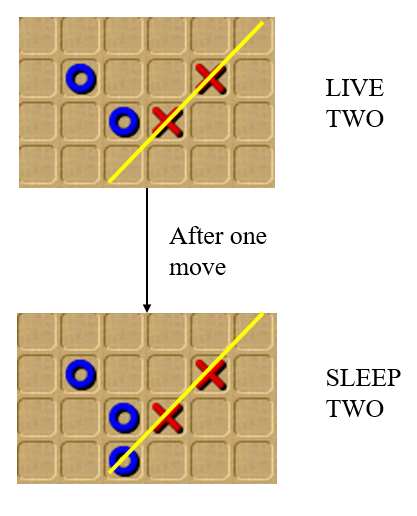
\includegraphics[width=0.28\textwidth]{figures/peer_update.png}
  \caption{An example for peer update}
  \label{fig:peer}
\end{figure}

%
As \autoref{fig:peer} shows, the two "\times" pieces consists the "live two" chess shape and both of them has 100 score in "v" direction.
%
After one move, an "o" piece is placed and the chess shape of those two "\times" pieces changed to "sleep two". Similarly, both of them has 10 score in "v" direction. 
%
It is not so difficult to observed that no matter how many moves are placed, in "v" direction, the two fixed adjacent "\times" chess would always have the same score. 
Such fixed adjacent chess with same color are called "Peer". 
All the peer chess would have the same score in relative direction and repeated calculations can be avoided.
%

%
In practice, the Peer Update algorithm scan the 
" {\ooalign{$\times$\cr\hidewidth$+$\hidewidth\cr}} "
from the center (the position of newly placed piece).
%
If the chess need to assign score is the same of the former one, it is unnecessary to compute the score and just assign the score of former one to the current one.
%

\subsection{Read Score in Dict.}


%
\quad In the midterm version, to get the score of specific chess shape,  lot of if-else judgments need to be made.
%
It is possible to store all the score related to the chess then such if-else judgments are not needed anymore.
%
In our version, the score are stored in a dictionary data structure.
%
It is noted that using a list may be the best choice because of the dictionary still need to do some extra hash computation.
%
However, the idea behind is similar and the implement of dictionary maybe much easier.
%

%
To distinguish chess shapes as finely as possible, a pentagon is used as a key to the dictionary.
%
Denoted the pentagon as $(a, b, c, d, e)$, the $a$ and $e$ denotes the block message. 
%
If it is outside the board or meet a opponent chess when searching from the center in positive direction, then $a$ is True and else False. 
%
$e$ is the same.
%
$c$ denotes the number of middle consecutive pieces, and $b$ and $d$ are the non-consecutive piece, the empty point could be tolerated is only one.
%


\begin{figure}[h]
  \centering
  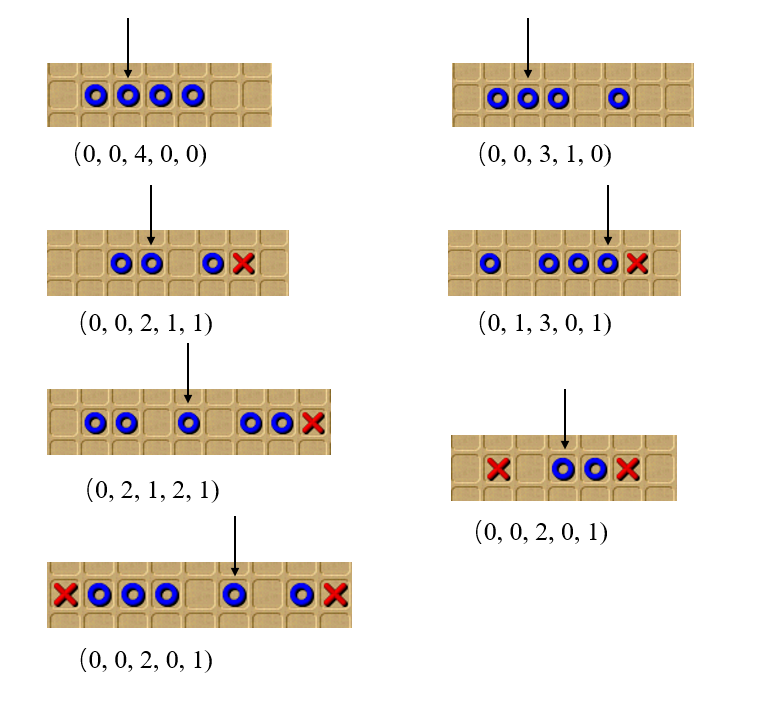
\includegraphics[width=0.4\textwidth]{figures/dict.png}
  \caption{Some examples for score dictionary}
  \label{fig:dict}
\end{figure}

%
It is apparent that the peer pieces
would have the same key.
%
This method to extract chess shape has advantage of covering some complex chess shape,
but its disadvantage is only one empty point tolerated that the search is limited.
%
For example, the "live one" chess shape only need one empty on both side instead of two in classical method.
%
Generally, reading score in dictionary could improve the performance of AI.

\subsection{Checkmate Search}
\quad Checkmate is a terminology for a lot of board games, which means your enemy does a move which you have to respond and take defensive measures, otherwise you will lose the game. 
%
In Gomoku, the existing of multiple checkmates makes it possible to appear must-win situation, double live three is such an example.
%
A winning threat sequence for a player is an action sequence which consists of a sequence of checkmate which leads to a must-win situation\cite{threat}.
%
If such a winning threat sequence exists in a fixed board state, we simply do moves in that sequence and can get a win.
%
However, in Allis and Herik's paper\cite{threat}, the whole technology is too complex to realize, so we implement a simplified version of winning threat space search, and name it checkmate search.

In our implementation, we maintain threat list recursively, and taking into considerate that the enemy is perfectly responding, i.e. he take defensive measures for sure, then we want to know whether it can leads to a must-win situation. 
%
For example, in \autoref{fig:checkmate}, assuming we are considering player "$\times$"'s checkmate.
%
Firstly, there are two points that can make chess shape "$sleep\ four$", and for the left move, if we do move like that, and the enemy do move as shown (he has to do move like that, or he will loss the game), there will have no checkmate move; else if we do move like right, the enemy do move as shown (he has to do move like that as well), there will have another two checkmate moves signed as $\textcircled{1}$ and $\textcircled{2}$, then we can recursively search after we do that move. 
\begin{figure}[h]
  \centering
  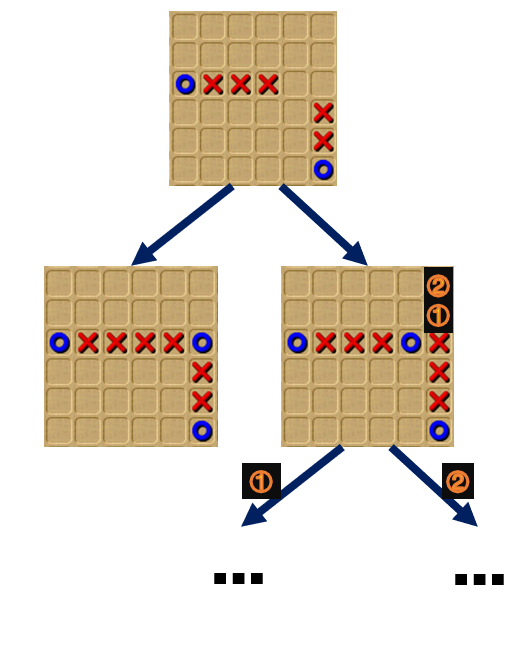
\includegraphics[width=0.3\textwidth]{figures/checkmate.png}
  \caption{An example for "$\times$"'s checkmate}
  \label{fig:checkmate}
\end{figure}

To prevent timeout, a upper bound for the checkmate search's depth should be applied, in practice, we set the max checkmate search's depth as 16. 
%
It is worth noting that, the checkmate search is much quicker than minimax search, because its brunch factor is always small. 
%
Meanwhile, the checkmate search can be not only used for the agent, but also used for its enemy, checking whether its enemy have a winning threat sequence can help the agent to avoid some bad moves in advance. 



\section{Monte Carlo Tree Search}
\quad Monte Carlo Tree Search (MCTS) is a series of algorithms. This kinds of algorithms can explore huger space than any other tree search algorithms. Meanwhile, this kinds of algorithms often requires a large number of simulation, and the more simulation time it does, the more accurate it will perform.  The basic process of MCTS consists four main steps: Selection, Expansion, Simulation, and Backpropagation.

At first stage Selection, it begins from the root node, and applies Tree Policy to select a child which is the most worthwhile expandable. Then at Expansion stage, it will add a child node for the selected node to expand the tree according to the available actions. At the third stage Simulation, it will simulate a whole chess game, and at the leaf node will produce an outcome, i.e. win or loss. Finally, at Backpropagation stage, it will back propagate the simulation result from the expanded nodes to the root node, to update their state values. An example of the basic process of MCTS is shown in \autoref{fig:mcts}.


\begin{figure*}
  \centering
  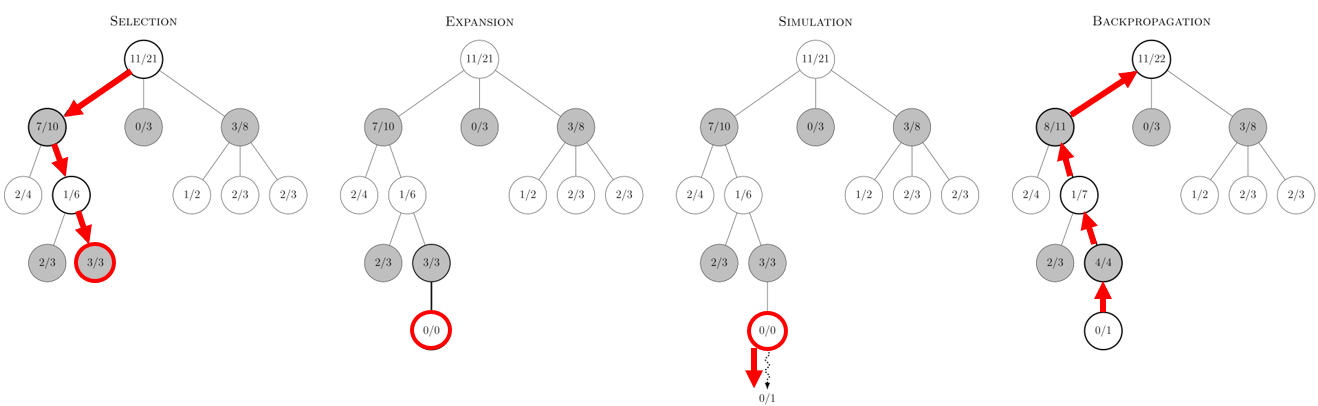
\includegraphics[width=\linewidth]{figures/mct.png}
  \caption{An example for basic process of MCTS}
  \label{fig:mcts}
\end{figure*}

\subsection{HMCTS}
\quad We implement two kinds of MCTS algorithms in this report. One is called Heuristic Monte Carlo Tree Search (HMCTS), and the other is called Upper Confidence bounds for Tree (UCT). The HMCTS for Gomoku is presented in Algorithm 1.

\begin{breakablealgorithm}
\caption{\quad HMCTS for Gomoku}\label{Algorithm 1}
\begin{algorithmic}
\noindent \textbf{Input:} current board state $s_0$, simulation times T;\\
\noindent \textbf{Output:} best action $a$ according to the simulation result of MCTS;
\State
\State $M$ = Candidates($s_0$)
\For{each action $m$ in moves $M$}
    \State reward $r$ $\leftarrow$ 0;
    \State simulation time t $\leftarrow$ 0;
    \State $s(m)$ $\leftarrow$ $f(s_0, m)$;
    \While{t $<$ T}
        \State $r$ $\leftarrow$ $r$ + Simulation($s(m)$);
        \State t $\leftarrow$ t + 1;
    \EndWhile
    \State add ($m$, $r$) into $data$;
\EndFor\\
\Return{Best($data$)}
\State
\Function{Candidates}{board state $s$}
\For{all points $p$ which is not occupied}
	\If{$p$ is a neighbor of one point which is occupied}
	\State add $p$ into $candidates$;
	\EndIf
\EndFor
\State \Return{candidates}
\EndFunction


\State
\Function{Simulation}{board state $s_t$}
	\If{$s_t$ is terminal}
	    \If{AI win}
	    \State \Return{1.0}
	    \ElsIf{draw}
	    \State \Return{0.5}
	    \Else
	    \State \Return{0.0}
	    \EndIf
	\ElsIf{Heuristic($s_t$)}
	    \State $a_t$ $\leftarrow$ Heuristic($s_t$)
	    \State $s_{t+1}$ $\leftarrow$ $f(s_t, a_t)$
	    \State \Return{Simulation($s_{t+1}$)}
	\Else
	    \State $a_t$ $\leftarrow$ random action $\in$ untried actions
	    \State $s_{t+1}$ $\leftarrow$ $f(s_t, a_t)$
	    \State \Return{Simulation($s_{t+1}$)}
    \EndIf
\EndFunction

\State
\Function{Heuristic}{board state $s_t$}
\If{I have four-in-a-row}
    \State \Return{the point emerge five for me}
\ElsIf{The opposite has four-in-a-row}
    \State \Return{the point emerge five for opposite}
\ElsIf{I have three-in-a-row}
    \State \Return{the point emerge four for me}
\ElsIf{The opposite have three-in-a-row}
    \State \Return{the point emerge four for opposite}
\Else
    \State \Return{False}
\EndIf
\EndFunction

\State 
\Function{BEST}{$data$}
	\State \Return{action $a$}\quad //the maximum $r$ of $m$ in $data$
\EndFunction

\end{algorithmic}
\end{breakablealgorithm}

Note that in Algorithm 1, $f(s, a)$ is a function to generate a new board state according to the last board state and an action.
%
And the heuristic knowledge is commonly known among Gomoku players, which can save some time and make it more accuracy in simulation step than acting randomly. 

As for how to obtain heuristic information in our implementation, we maintain two $20\times 20$ hash tables, which store each point's maximal count for both white chess and black chess.
%
When the current board is given, first initialise the whole hash tables for each points, then while simulating, updating the hash tables step-wisely.
%
In stage simulation, when the heuristic information is needed, we can just simply check the two hash tables, recall that they store each point's maximal count for white chess or black chess. So if there exists some value $\geq$ 4 in the hash tables, it means that the heuristic information can be used.

For example, as shown in \autoref{fig:hashtable}, when initialising the two hash tables and taking into considerate the stared point, it will store 3 in "o"'s hash table (the maximal count appears at main diagonal direction), and store 2 in "x"'s hash table (the maximal count appears at column direction).

\begin{figure}[h]
  \centering
  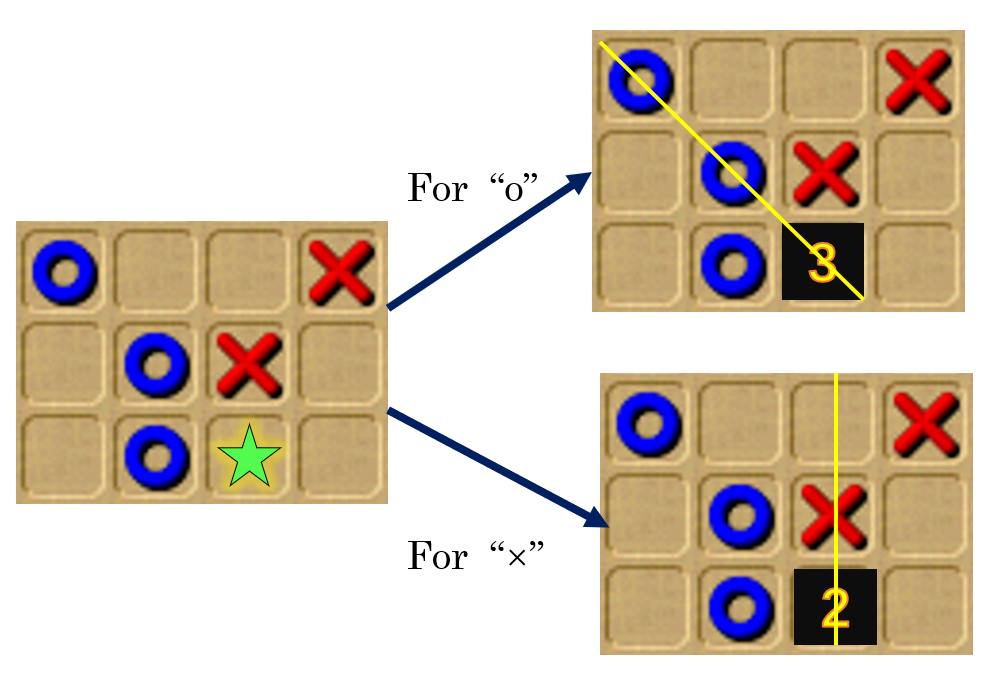
\includegraphics[width=0.38\textwidth]{figures/2.png}
  \caption{How do the hash tables work}
  \label{fig:hashtable}
\end{figure}


\subsection{UCT}
%
\quad UCT is another kind of MCTS algorithms, which is actually originated from HMCTS, but more time-saving and complex than HMCTS. 
%
Comparing HMCTS and UCT, it can be simply summarised as follows: HMCTS treat every possible actions equally, and simulate them the same times; while UCT treat different possible actions 'unfairly', and simulate different actions time-differently, it prior simulate the 'valuable' action in each simulation.
%
How do UCT measure the 'value' of a move is UCB, which is used to trade-off the exploration and exploitation, in each step, the agent select the child node which has the largest UCB value.
%
The UCB is defined as follows:
\begin{align*}
    UCB = \frac{Q_i}{n_i} + c\cdot \sqrt{\frac{ln(n)}{n_i}}\tag{1}
\end{align*}

Where $\frac{Q_i}{n_i}$ is the average reward for node $i$ after a simulation, $n$ is the total number of simulation times so far, $n_i$ is the number of times that node $i$ is visited. Meanwhile, $c$ is a positive parameter, and in practice, we set $c = \sqrt{2}$.

Also, in this formula, The average reward $\frac{Q_i}{n_i}$ encourages the exploitation of higher reward selection, but $\sqrt{\frac{ln(n)}{n_i}}$ encourages the exploration of less visited choices. So by using the UCB, the UCT algorithm balance the exploration and exploitation.
%
Our implementation of UCT is presented in Algorithm 2.


\begin{breakablealgorithm}
	\caption{\quad UCT for Gomoku}\label{Algorithm 2}
	\begin{algorithmic}
	\noindent \textbf{Input:} root state $s_0$, simulation times T; parameter $c$\\
    \noindent \textbf{Output:} best action $a$ according to the simulation result;
    \State
	\State simulation time t $\leftarrow$ 0;
    \While{t $<$ T}
    \State $s_l$ $\leftarrow$ TreePolicy($s_0$)
        \State reward $r$ $\leftarrow$ Simulation($s_l$);
        \State BackPropagation($s_l$, $r$)
    \EndWhile
    \State \Return{BestChild($s_0$)}
	\State
	\Function{TreePolicy}{node $s$}
		\While{$s$ is not leaf}
			\If{$s$ not fully expanded}
				\State \Return{Expend($s$)}
			\Else
				\State $s$ $\leftarrow$ BestChild($s$, $c=\sqrt{2}$)
			\EndIf
		\EndWhile
		\State \Return{$s$}
	\EndFunction
	\State
	\Function{BackPropagation}{node $s$, reward $r$}
		\While{$s.parent$ is not None}
			\State $s.visit_time$ $\leftarrow$ $s.visit_time$ + 1
			\State $s.Q$ $\leftarrow$ $s.Q$ + $r$
			\State $s$ $\leftarrow$ $s.parent$
		\EndWhile
	\EndFunction
	\end{algorithmic}
\end{breakablealgorithm}

Note that in Algorithm 2, function $Simulation$ is the same as Algorithm 1, function $BestChild(s, c)$ returns a child of $s$ with the largest UCB value, and function $Expend(s)$ is a function add a possible move into the board state $s$ and generate a new state.
%
And the heuristic knowledge is commonly known among Gomoku players, which can save some time and make it more accuracy in simulation step than acting randomly. 

Meanwhile, we also maintain two $20\times 20$ hash tables to obtain heuristic information in our implementation. Recall that two hash tables store each point's maximal count for both white chess and black chess.

\section{Adaptive Dynamic Programming}
%
\quad As what we have learn in course, Reinforcement Learning (RL)  is to learn how to map an action to a state to get the maximal reward from interacting with the environment. 
%
During the learning process, no explicit teacher is needed.
%
Temporal Difference (TD) learning is a classical model-free reinforcement learning methods, which learn by bootstrapping from the current estimate of the value function. 
%
As Tang\cite{Tang/ztt} claims, the action 
decision or the value function could also be described in a 
continuous form in TD, which is the the core idea of Adaptive Dynamic 
Programming (ADP).

%
Our version of ADP based on the framework of Zhao\cite{Zhao/ztt}, consists of three parts: Critical Network, Action Network and System Model.

%% 将三部分的图放在此处。
\begin{figure}[h]
  \centering
  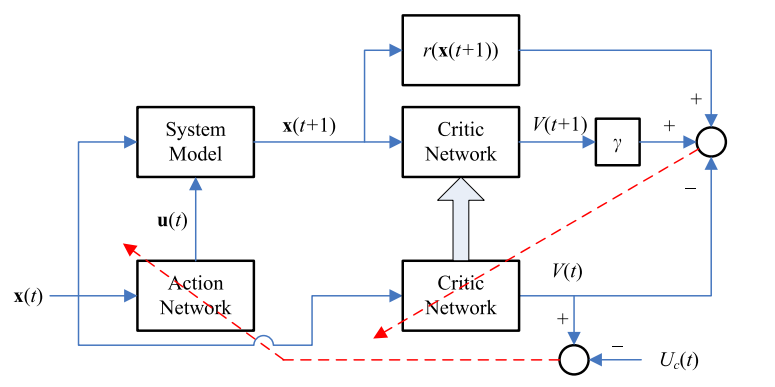
\includegraphics[width=0.5\textwidth]{figures/ADP.png}
  \caption{The Process of ADP}
  \label{fig:adp}
\end{figure}


\subsection{The State}
%
\quad To evaluate a board situation, the important issue is how to
choose the proper features.
%
Zhao's work carefully choose 20 patterns for each of the two players.
%
However, such method need to deepcopy the board state for every move and scan the whole board to extract features.
%

%
To be consistent with the former framework using in $\alpha-\beta$ game search (midterm version), point update methods are still used to maintain board status.
%
Because of the lack of depth research about point update method, all the 100 chess shape are considered to described the board the state.
%
To present the state of a board, the number of point belongs to each chess shape would be counted.
%
In addition, whose turn to move is another important piece of
information for describing a board situation.

\subsection{System Model}
%
\quad The system model presents that how the state of board changes board and given rewards to the AI players.
%
Since the fast update method is introduced, the state of board would be updated by Point Update quickly.
%
Concerning the rewards, no rewards would be given during the game.
%
After a game, if AI player wins, the final reward is 1, if he loses, the reward is 0, and if he draws against his opponent, the reward
is 0.5.
%


\subsection{Critical Network}
%
\quad A feed-forward three-layered fully connected neural network is adopted to evaluate board situations.
%

%
For each chess shape, two input nodes to present the number of point for two player respectively.
%
Other two input nodes are assign to represent the turn for each chess shape as well.
%
If AI itself moves first, then the first input is 1 and the second input is 0.
%
If opponent player moves first, then the inputs for these two nodes are reverted.
%
Also, two nodes presenting the turn for the whole board is needed.
%
Therefore, the number of input nodes adds up to $100*(2+2)+2 = 402$.

%
In our design, there are 402 nodes in the input layer, 64 nodes in the
hidden layer and 1 node in the output layer.
%
The output of the neural
network is the winning probability of AI player starting from a
board situation.
%

\subsection{Action Network}
%
\quad As is mentioned in the midterm report, there are many accurate and approximate reductions to choose the next move.
%
To make the AI player implied by pure ADP, those reductions based on heuristic functions are abandoned.
%
The only reduction taken is that the points are considered only if which is 
near a position which has been occupied.
%
During the training process, when there are several alternative actions which have equally high evaluation, we simply choose the
one that is first found.
%

%
To cope with the exploration–exploitation dilemma,
the state space of Gomoku are explored in the ways below.
%
For the first move, the AI player randomly choose a position to start.
%
For the rest moves, a $\epsilon-$greedy policy is applied for both players, which is defined as follows.

$$ y=\left\{
\begin{aligned}
&\arg \max_\alpha\ V(t+1) &\text{with probability 1 - }\epsilon \\
&\text{random action} &\text{with probability }\epsilon
\end{aligned}
\right.
$$

%
With the number of training games increasing, the value of e should decrease gradually.
%







\section{Experimental Results}
\subsection{Performance}
\quad We do experiments for $\alpha-\beta$ pruning, ADP, HMCTS, UCT between four different Gomoku AIs: mushroom, fiverow, valkyrie and Pisq. Each plays 6 games (three different openings and first/second hand) with the four AIs, and the result is shown as follows.
\begin{table}[h]
\caption{Results for different agents}
    \centering
    \label{table1} 
    \begin{tabular}{|c|c|c|c|c|}
    \hline
    $Agent$&mushroom&fiverow&valkyrie&Pisq\\
    \hline
    $\alpha\beta$-7&6:0&6:0&6:0&5:1\\
    \hline
    HMCTS-10&6:0 &4:2 &2:4 &1:5 \\
    \hline
    UCT-10&4:2 &3:3 &1:5 &0:6 \\
    \hline
    ADP& 3:3&2:4 &0:6 &0:6 \\
    \hline
    \end{tabular}
\end{table}

It can be found that depth-7 $\alpha-\beta$ pruning performs pretty well, as to MCTS algorithms, HMCTS performs better than UCT from the result. Meanwhile, both of them However, the ADP doesn't perform as we expected, but we believe that maybe it need a little more training time, and that can make a smarter agent.


\subsection{Time Consuming}
\quad In the experiments above, we recorded the time spent at the same time. The average time-spending results for per move are shown as follows :
\begin{table}[h]% h asks to places the floating element [h]ere.
  \caption{Time-spending results (unit: second)}
  \label{tab:freq}
  \begin{tabular}{cccc}
    \toprule
     $\alpha\beta$-7&HMCTS-10&UCT-10&ADP\\
    \midrule
    2.96 & 29.1 & 1.49& 0.016\\
  \bottomrule
\end{tabular}
\end{table}

It can be found that fter our optimization for $\alpha-\beta$ pruning, it can do move quickly even in a depth-7 search tree. At the same time, compared with UCT, HMCTS is too slow to do one move, so it can not become a qualified Gomoku AI player. Meanwhile, as a neural network product, ADP moves so fast for each step.

\section{Conclusions and Future Work}

%%% future work, 需要谈Limitations吗
\quad So far, we implemented several Gomoku AIs by using MCTS (HMCTS and UCT), ADP, and improved the $\alpha$-$\beta$ pruning by adding some new technologies.
%
And as a result, we finally get at most 1447 rating under Bayesian Elo.

As we known, by now, the best AI agent playing Gomoku around the world is based the method of neutral network and ADP.
%
However, according to the lack of enough knowledge of neutral network and the limitation of training time and machine, the performance of our ADP is not so good.
%
It maybe necessary to design the state presentation as well as the critical network structure carefully and to apply some technique to speed up the training process in the future study.

Meanwhile, for $\alpha-\beta$ pruning, after we read some open source code for some strong AI with high score, for example, pela, they use a novel framework, which maintain a 256 $\times$ 256 matrix-like hash table to evaluate the point in the chess board. 
%
In each position of the hash table is indexed by an abscissa and an ordinate to get the point value, and the abscissa is determined by the chess shape of our agent, the ordinate is determined by the chess shape of its enemy's. 
%
Both of the chess shape is read by an 8-bit binary number: the low 4 bits and the high 4 bits are in opponent positions of the evaluating point. It is such a good frame work that can further accelerate. 

But after all, this is not our own thought, and we believe in our own framework, we have done the best.
%\clearpage










\bibliographystyle{ACM-Reference-Format}
\bibliography{sample}

\end{document}
\endinput
